\section{Background}\label{sec:background}

\subsection{Description of AES}\label{sub:description_cipher}

%\paragraph{}
%citation for the aes specification
AES~\cite{AES} is a 128-bit block cipher, designed by Rijmen and Daemen in 1997 (originally, under the name Rijndael). In 2001, it was selected by the US National Institute of Standards (NIST) as the Advanced Encryption Standard, and since then, it has gradually become the most widely used block cipher worldwide. 

AES is a Substitution-Permutation Network operating on a 128-bit state organized as a $4\times4$ array of 8-bit words. The encryption process is composed of 10, 12, or 14 rounds (depending on the key length: 10 rounds for 128-bit keys, 12 rounds for 192-bit keys, and 14 rounds for 256-bit keys). Each round of AES is composed of four operations, presented in Figure~\ref{fig:AESRound}: 
\begin{itemize}[leftmargin=.02in]
    \item[] \textbf{\subB}. Apply a known 8-bit S-box independently to the bytes of the state; 
    \item[] \textbf{\sr}. Shift each row of the state to the left by the position of the row;
    \item[] \textbf{\mc}. Multiply each column by the same known invertible 4-by-4 matrix over the finite field $GF(2^8)$;
    \item[] \textbf{\ak}. Add a 128-bit round key computed from the secret key to the state, using a bitwise XOR operation.
%Apply independently the following MDS transformation 
%    $\begin{pmatrix} 
%        2 & 3 & 1 & 1 \\
%        1 & 2 & 3 & 1 \\
%        1 & 1 & 2 & 3 \\
%        3 & 1 & 1 & 2
%    \end{pmatrix}$ to each column of the state in $\textsc{GF}(2^8)$.
\end{itemize}
%\VM{see if this is the best way to define the round in relation to what we will do in the partial sum}
%The round function is repeated 10, 12 and 14 respectively for 128, 192 and 256-bit keys. 
An additional \ak operation is applied before the first round, and
the last \mc operation is omitted. As properties of the key schedule of AES are not used in this paper, we refer the reader to~\cite{AES} for its description.

\begin{figure}
\vspace*{-1.1cm}
\begin{center}
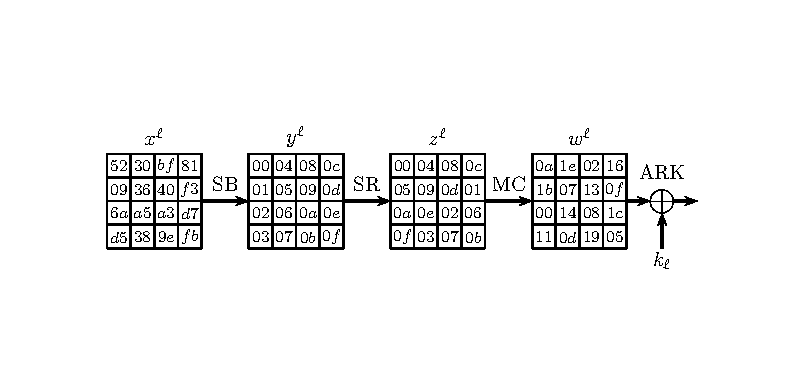
\includegraphics[trim = 10em 8em 10em 4em]{fig/AES-round.pdf}    
\end{center}
\caption{An AES Round}\label{fig:AESRound}
%\vspace*{-0.6cm}
\end{figure}

The rounds are numbered from $0$ to $Nr-1$, where $Nr$ is the number of rounds. The subkey used in the \ak operation of round~$\ell$ is denoted by $k^{\ell}$, and the $j$'th byte in its $i$'th row is denoted by $k^{\ell}_{4j+i}$. The whitening key added before the initial round is denoted by $k^{-1}$. The $j$'th byte in the $i$'th row of the state before the \subB, \sr, \mc, \ak operations of round~$\ell$ is denoted by $x^\ell_{4j+i}, y^\ell_{4j+i}, z^\ell_{4j+i},$ and $w^\ell_{4j+i}$, respectively.  A set of bytes $\left\{v_i, v_j, v_k\right\}$ is denoted by $v_{i,j,k}$.

\subsection{The Square Attack on AES}
\label{sec:sub:Square}

AES was designed as a modification of the block cipher Square~\cite{FSE:DaemenKR97}, which came together with a dedicated attack, called `the Square attack'. This attack, in its basic application to AES, uses the following observation.
\begin{lemma}\label{Lem:Square1}
Consider the encryption by 3-round AES of a set of 256 plaintexts, $P_0,P_1,\ldots,P_{255}$, which are equal in all bytes except for a single byte, such that the single byte assumes each possible value exactly once. Then the corresponding ciphertexts $C_0,C_1,\ldots,C_{255}$ satisfy $\bigoplus_{i=0}^{255} C_i=0$.  
\end{lemma}
As was shown in~\cite{FSE:DaemenKR97}, this property can be used to attack 6-round Square, and also 6-round AES, with a complexity of about $2^{80}$ S-box computations. The adversary asks for the encryption of $2^{32}$ plaintexts which are equal in all bytes except for the main diagonal (i.e., bytes 0,5,10,15) and assume all $2^{32}$ possible values in the main diagonal. Then, he guesses bytes $0,5,10,15$ of $k^{-1}$, and for each guess, he partially encrypts the plaintexts through round~0 and finds a set of $2^8$ inputs to round~1 which satisfy the assumption of Lemma~\ref{Lem:Square1}. Then, he partially guesses the subkeys $k^4,k^5$, partially decrypts the $2^8$ corresponding ciphertexts through rounds~4,5 and checks whether the XOR of the $2^8$ corresponding values at the state $x^4_0$ (i.e., at byte 0 before the \subB operation of round~4) is zero, as is stated by Lemma~\ref{Lem:Square1}. If not, the subkey guess is discarded.

While it seems that in order to compute byte $x^4_0$ from the ciphertext, the adversary must know 64 subkey bits (specifically, key bytes $k^5_{0,7,10,13}$ and $k^4_{0,1,2,3}$), in fact knowing 40 subkey bits is sufficient. Indeed, since \mc is a linear operation, it can be interchanged with the \ak operation after it, at the cost of replacing $k^4$ with the equivalent subkey $\bar{k}^4=\mc^{-1}(k^4)$. The knowledge of the key bytes $k^5_{0,7,10,13}$ and $\bar{k}^4_0$ is sufficient for computing the state byte $x^4_0$ from the ciphertext of 6-round AES.\footnote{Here and in the sequel, we assume that in 6-round AES, the \mc operation of round~5 is omitted. If this operation is not omitted, the attack works almost without change; we only have to replace the key $k^5$ with the equivalent key $\bar{k}^5=\mc^{-1}(k^5)$.} Each check whether $2^8$ values XOR to zero provides an 8-bit filtering, and hence, checking several sets is sufficient for discarding all wrong subkey guesses. The attack recovers 9 subkey bytes ($k^{-1}_{0,5,10,15},\bar{k}^4_0,k^5_{0,7,10,13}$) with complexity of about $2^{32} \cdot 2^{40} \cdot 2^8=2^{80}$ S-box computations.

In~\cite{FSE:FKLSSWW00}, Ferguson et al.~observed that the Square attack can be improved by replacing Lemma~\ref{Lem:Square1} with the following lemma on 4-round AES.
\begin{lemma}\label{Lem:Square2}
Consider the encryption by 4-round AES of a set of $2^{32}$ plaintexts, $P_0,P_1,\ldots,P_{2^{32}-1}$, which are equal in all bytes except for the main diagonal (i.e., bytes 0,5,10,15), such that the diagonal assumes each possible value exactly once. Then the corresponding ciphertexts $C_0,C_1,\ldots,C_{2^{32}-1}$ satisfy $\bigoplus_{i=0}^{2^{32}-1} C_i=0$.  
\end{lemma}
Lemma~\ref{Lem:Square2} can be used to attack 6-round AES using the same strategy described above. The adversary asks for the encryption of a few sets of $2^{32}$ plaintexts which satisfy the assumption of Lemma~\ref{Lem:Square2}. Then, for each set, he guesses subkey bytes $\bar{k}^4_0,k^5_{0,7,10,13}$ and checks whether the XOR of the $2^{32}$ intermediate values at the state byte $x^4_0$ is zero, as is stated by Lemma~\ref{Lem:Square2}. The attack recovers 5 subkey bytes ($\bar{k}^4_0,k^5_{0,7,10,13}$) and its complexity is about $2^{32} \cdot 2^{40}=2^{72}$ S-box computations.

\subsection{The Partial Sums Attack}
\label{sec:sub:partial-sums}

In the same paper~\cite{FSE:FKLSSWW00}, Ferguson et al.~showed that the complexity of the Square attack described above can be significantly reduced, by dividing the key guessing and partial decryption into several steps and gradually reducing the number of values whose XOR should be computed. By the structure of AES, the state byte $x^4_0$ is computed from the ciphertext $C$ using the following formula:
\begin{align}\label{Eq:Square1}
  \begin{split}
x^4_0=S^{-1}\big(\bar{k}^4_0 \oplus \hex{0e} \cdot &S^{-1}(C_0 \oplus k^5_0) \oplus \hex{09} \cdot S^{-1}(C_7 \oplus k^5_7) \oplus \\
&\oplus \hex{0d} \cdot S^{-1}(C_{10} \oplus k^5_{10}) \oplus \hex{0b} \cdot S^{-1}(C_{13} \oplus k^5_{13})\big),
  \end{split}  
\end{align}
where the coefficients $\hex{0e},\hex{09},\hex{0d},\hex{0b}$ come from the inverse \mc operation and the multiplication is performed in the finite field $GF(2^8)$. 

Note that the right hand side of~\eqref{Eq:Square1} depends only on bytes 0,7,10,13 of the ciphertext. This means that if two ciphertexts are equal in these four bytes, then their contributions to the XOR of $x^4_0$ values cancel each other. Thus, we may replace the list of ciphertexts with a list $A$ of $2^{32}$ binary indices which indicates whether each of the $2^{32}$ possible values of bytes 0,7,10,13 of the ciphertext appears an even or an odd number of times in the list of ciphertexts. The goal of the subsequent steps is to reduce the number of needed binary indices, in parallel to guessing subkey bytes. 

At the first step, the adversary guesses bytes 0,7 of $k^5$, and reduces the size of the list to $2^{24}$. Denote $a_1 = \hex{0e} \cdot S^{-1}(C_0 \oplus k^5_0) \oplus \hex{09} \cdot S^{-1}(C_7 \oplus k^5_7)$. Observe that if two ciphertexts are equal in the bytes $a_1,C_{10},C_{13}$, then their contributions to the XOR of $x^4_0$ values cancel each other. As the guess of bytes $k^5_{0,7}$ allows computing $a_1$ for each ciphertext, the adversary can construct a list $A_1$ of $2^{24}$ binary values which indicates whether each possible value of $(a_1,C_{10},C_{13})$ appears an even or an odd number of times in the list of intermediate values. The complexity of this step is about $2^{16} \cdot 2^{32}=2^{48}$ S-box evaluations.

At the second step, the adversary guesses the byte $k^5_{10}$ and reduces the list to a list $A_2$ of size $2^{16}$ that corresponds to the possible values of $(a_2,C_{13})$, where $a_2 = a_1 \oplus \hex{0d} \cdot S^{-1}(C_{10} \oplus k^5_{10})$. At the third step, the adversary guesses the byte $k^5_{13}$ and reduces the list to a list $A_3$ of size $2^{8}$ that corresponds to the possible values of $a_3$, where $a_3 = a_2 \oplus \hex{0b} \cdot S^{-1}(C_{13} \oplus k^5_{13})$. Finally, at the fourth step, the adversary guesses the byte $\bar{k}^4_0$, computes $\oplus_{\{x \in \{0,1\}^8:A_3[x]=1\}} S^{-1}(\bar{k}^4_0 \oplus x)$, which is equal to the right hand side of~\eqref{Eq:Square1}, and checks whether it is equal to zero. The complexity of each step is about $2^{48}$ S-box computations, and thus, the overall complexity for a single set of $2^{32}$ plaintexts is $2^{50}$ S-box computations. 

As the attack recovers 5 subkey bytes, six sets of $2^{32}$ plaintexts are required to recover their value uniquely with a high probability. Note that after the check of the first set, only about $2^{40} \cdot 2^{-8}=2^{32}$ suggestions for the 40 subkey bits remain undiscarded. This means that for each possible value of $k^5_{0,7,10,13}$, at most a few values of $\bar{k}^4_0$ that correspond to them are expected to remain. Hence, when examining the second set of $2^{32}$ plaintexts, the complexity of the fourth step becomes negligible as it is performed only for a few values of $\bar{k}^4_0$. Similarly, when examining the third set, the two last steps become negligible, etc. In total, the complexity of checking all six plaintext sets of size $2^{32}$ is equivalent to the cost of $4+3+2+1=10$ steps, or $2^{51.3}$ S-box computations.\footnote{We note that in~\cite{FSE:FKLSSWW00}, the authors performed a similar analysis and concluded that the complexity is $2^{52}$ S-box computations. This value was used in all subsequent papers. For the sake of consistency, we use the same value in Table~\ref{Tab:Results}, but note that the actual complexity is lower, as is shown here, and use the lower estimate when comparing the partial sums attack with our new attack.} 

The attack is given as Algorithm~\ref{alg:partial-sum}.
To simplify the notation, we rewrite equation~\eqref{Eq:Square1} in a more generic way, using
$S_0$ for $\hex{0e} \cdot S^{-1}(\cdot)$,
$S_1$ for $\hex{09} \cdot S^{-1}(\cdot)$,
$S_2$ for $\hex{0d} \cdot S^{-1}(\cdot)$,
$S_3$ for $\hex{0b} \cdot S^{-1}(\cdot)$,
and renaming the keys and the ciphertext bytes to $k_0, k_1, k_2, k_3, k_4$ and $c_0, c_1, c_2, c_3$, respectively:
\begin{equation}
    a_4 = S^{-1}\left(k_4 \oplus S_0(c_0 \oplus k_0) \oplus S_1(c_1 \oplus k_1) \oplus S_2(c_2 \oplus k_2) \oplus S_3(c_3 \oplus k_3)\right).
    \label{Eq:Square2}
\end{equation}

\begin{algorithm}[!ht]
    \begin{algorithmic}[1] % enter the algorithmic environment
        \State Input: Array $A$ of bits such that the $j^{\text{th}}$ value of $A$ denotes the parity of the number of occurrences of $j$ in the list of ciphertexts
            \ForAll{$k_0, k_1$}
            \State Declare an empty bit-array $A_1$ of size $2^{24}$
                \ForAll{$c_0, c_1, c_2, c_3$}
                    \If{$A[c_0, c_1, c_2, c_3] = 1$}
                        \State{$a_1 \gets S_0(c_0 \oplus k_0) \oplus S_1(c_1 \oplus k_1)$}
                        \State{$A_1[a_1, c_2, c_3] \gets A_1[a_1, c_2, c_3] \oplus 1$}
                    \EndIf
                \EndFor

                \ForAll{$k_2$}
                    \State Declare an empty bit-array $A_2$ of size $2^{16}$
                    \ForAll{$a_1, c_2, c_3$}
                        \If{$A_1[a_1, c_2, c_3] = 1$}
                            \State{$a_2 \gets a_1 \oplus S_2(c_2 \oplus k_2)$}
                            \State{$A_2[a_2, c_3] \gets A_2[a_2, c_3] \oplus 1$}
                        \EndIf
                    \EndFor

                    \ForAll{$k_3$}
                        \State Declare an empty bit-array $A_3$ of size $2^{8}$
                        \ForAll{$a_2, c_3$}
                            \If{$A_2[a_2, c_3] = 1$}
                                \State{$a_3 \gets a_2 \oplus S_3(c_3 \oplus k_3)$}
                                \State{$A_3[a_3] \gets A_3[a_3] \oplus 1$}
                            \EndIf
                        \EndFor

                        \ForAll{$k_4$}
                            \State {$a_4 \gets 0$}
                            \ForAll{$a_3$}
                                \If{$A_3[a_3] = 1$}
                                    \State $a_4 \gets a_4 \oplus S^{-1}(k_4 \oplus a_3)$
                                \EndIf
                            \EndFor
                            \If{$a_4 \ne 0$}
                                \State {$k_0, k_1, k_2, k_3, k_4$} is not a valid key candidate
                            \EndIf
                        \EndFor
                    \EndFor
             \EndFor
            \EndFor
    \end{algorithmic}
\caption{Partial-sum algorithm for key recovery~\cite{FSE:FKLSSWW00}.\label{alg:partial-sum}}
\end{algorithm}


\paragraph{Reducing the data complexity.} In~\cite{Tunstall12}, Tunstall observed that the data complexity of the attack can be reduced to $2^{33}$ chosen plaintexts by examining two sets of $2^{32}$ plaintexts instead of six sets. The idea is to check an analogue of Equation~\eqref{Eq:Square1} for three additional bytes -- $x^4_5, x^4_{10},$ and $x^4_{15}$ -- using the same set of $2^{32}$ plaintexts. Note that in order to compute each of these three bytes from the ciphertext, the adversary needs the subkey bytes $k^{5}_{0,7,10,13}$ (which are the same as in Equation~\eqref{Eq:Square1}), along with a different byte of $\bar{k}^4$. When two sets are checked at the same byte, they provide a 16-bit filtering, which in particular yields an 8-bit filtering on the value $k^{5}_{0,7,10,13}$ which is common to all examined bytes. Hence, information from different bytes can be combined to recover $k^5_{0,7,10,13}$ with a high probability. 

The data complexity can be further reduced to $2^{32}$ by examining a single set and checking the XOR in all 16 bytes of $x^4$. The algorithm is more complex and uses a meet-in-the-middle procedure based on the properties of the AES key schedule. We omit the description here, as it will not be needed in the sequel. 

In~\cite{Tunstall12}, it is claimed that when the same set of plaintexts is used to check the parity in several bytes, the complexity of checking the first byte is dominant, as some of the computations performed for computing the XOR in different bytes are identical. However, this claim seems incorrect, as in the variant of Equation~\eqref{Eq:Square1} for other bytes, the order of the coefficients 
$\hex{0e},\hex{09},\hex{0d},\hex{0b}$ which stems from the inverse \mc operation is changed, and hence, the operations performed for different bytes are not identical and only knowledge of subkeys can be `reused'. Therefore, the complexity of the attack that uses two sets is about $(4+3+2+2+1+1)\cdot 2^{48}=2^{51.7}$ S-box computations, and the attack that uses one set takes about $16 \cdot 2^{50}=2^{54}$ S-box computations.

The idea of using two sets of size $2^{32}$ instead of six was independently suggested in~\cite{alda2016implementation} by Alda et al., who also verified it experimentally.

%\subsection{Integral attacks against AES with partial sums}\label{sub:literature_partial_sum}

\iffalse
\NK{
Here is the list of the papers we directly compete with. Of course, we will have to explain exactly our gain over each of them.
\begin{itemize}
    \item[\cite{FSE:FKLSSWW00}] Ferguson, Kelsey, Lucks, Schneier, Stay, Wagner, and Whiting, Improved cryptanalysis of Rijndael, FSE 2000.
    \\The basic "partial sums" paper.\\
    \item[\cite{Tunstall12}] Tunstall, Improved “Partial Sums”-based Square Attack on AES, SeCrypt 2012, eprint:2012/280
    \\Claims that "partial sums" on 6-round AES can be improved by a factor of 2, by examining only two $\delta$-sets instead of 6 in the original paper. Also claims that a single $\delta$-set is sufficient, if the memory is increased to $2^{40}$. How does this compare to / combine with our results?\\
    \SG{Did not understand it completely, but if we can use it in our attack, we transform a $\times 6$ factor into a $\times 2$ in the overall complexity.}
    \item[\cite{EPRINT:AANS14}] Alda, Aragona, Nicolodi, and Sala, Implementation and Improvement of the Partial Sum Attack on 6-round AES, Physical and Data-Link Security Techniques for Future Communication Systems, 2016, eprint:2014/216
    \\Claims that "partial sums" on 6-round AES can be improved by a factor of 2, by examining only two $\delta$-sets instead of 6. The attack was practically verified. How does this compare to / combine with our results? 
\end{itemize}
}
\fi

\subsection{The FFT-Based Attack of Todo and Aoki}
\label{sec:sub:FFT-old}

The general idea of using the Fast Fourier Transform (FFT) for speeding up cryptanalytic attacks on block ciphers goes back to Collard et al.~\cite{ICISC:CollardSQ07} who used the FFT to speed up linear cryptanalysis. This idea was extended to several other techniques, including multi-dimensional linear attacks~\cite{ACISP:NguyenWWL10,ACISP:NguyenWW11}, zero-correlation attacks~\cite{SAC:BGWWC13}, differential-linear attacks~\cite{C:BeierleLT20}, etc.
%
In~\cite{CANS:TodAok14}, Todo and Aoki proposed to replace the partial sums technique by an FFT-based technique. The basic idea behind the Todo-Aoki technique is that the sum of the values in the right hand side of Equation~\eqref{Eq:Square1} which we want to compute can be written in the form of a \emph{convolution} of tailor-made functions, as seen in Algorithm~\ref{alg:fht-todo}. 

Consider a set $S$ of $2^{32}$ ciphertexts for which we want to compute the XOR of the intermediate values at the state byte $x^4_0$. Like in the partial sums attack, denote by $A$ a bit array of size $2^{32}$, such that $A(c_0,c_1,c_2,c_3)=1$ if and only if $C_{0,7,10,13}=(c_0,c_1,c_2,c_3)$ holds for an odd number of ciphertexts in $S$. Let $f:\{0,1\}^{32} \to \{0,1\}$ be the indicator function of the array, that is, $f(c_0,c_1,c_2,c_3)=\indic(A(c_0,c_1,c_2,c_3)=1)$. Assume that the subkey $k_4$ was guessed, and let $g_i:\{0,1\}^{32} \to \{0,1\}$, for $0\leq i \leq 7$, be defined by 
%\begin{align}\label{Eq:Fourier1}
%  \begin{split}
%g_i(t_0,t_1,t_2,t_3)=[S^{-1}(\bar{k}^4_0 \oplus \hex{0e} \cdot &S^{-1}(t_0) \oplus \hex{09} \cdot S^{-1}(t_1) \oplus \\
%&\oplus \hex{0d} \cdot S^{-1}(t_2) \oplus \hex{0b} \cdot S^{-1}(t_3))]_i,
%  \end{split}  
%\end{align}
\begin{equation}\label{Eq:Fourier1}
g_i(t_0,t_1,t_2,t_3)=\left[S^{-1}\left(k_4 \oplus S_0(t_0) \oplus S_1(t_1) \oplus
S_2(t_2) \oplus S_3(t_3)\right)\right]_i,
\end{equation}
where $[S^{-1}(t)]_i$ denotes the $i$'th bit of $S^{-1}(t)$. Then, denoting by $[x(C,k_0,k_1,k_2,k_3)]_i$ the $i$'th bit of the value $x^4_0$ corresponding to the ciphertext $C$ for a given guess of $k_0,k_1,k_2,k_3$ (see Equation~\eqref{Eq:Square2}), we have
%\begin{align}
%    \begin{split}
%    \bigoplus_{C \in S} &[x^4_0(C)]_i = \bigoplus_{\{(c_0,c_1,c_2,c_3):A[c_0,c_1,c_2,c_3]=1\}} g_i(c_0 \oplus k_0,c_1 \oplus k_1,c_2 \oplus k_3, c_3 \oplus k_4) \\
%    &= \bigoplus_{(c_0,c_1,c_2,c_3) \in \{0,1\}^{32}} f(c_0,c_1,c_2,c_3) g_i(c_0 \oplus k^5_0,c_1 \oplus k^5_7,c_2 \oplus k^5_{10}, c_3 \oplus k^5_{13}) \\
%    &= (f * g_i)(k^5_0,k^5_7,k^5_{10},k^5_{13}).
%    \end{split}
%\end{align}
\begin{align}
\begin{split}
    \bigoplus_{C \in S} \left[x(C,k_0,k_1,k_2,k_3)\right]_i
    &= \bigoplus_{\mathmakebox[6em][c]{\{(c_0,c_1,c_2,c_3):A[c_0,c_1,c_2,c_3]=1\}}} g_i(c_0 \oplus k_0,c_1 \oplus k_1,c_2 \oplus k_2, c_3 \oplus k_3) \notag \\
    &= \bigoplus_{\mathclap{c_0,c_1,c_2,c_3}} f(c_0,c_1,c_2,c_3) \cdot g_i(c_0 \oplus k_0,c_1 \oplus k_1,c_2 \oplus k_2, c_3 \oplus k_3) \\
    &= (f * g_i)(k_0,k_1,k_2,k_3).
\end{split}
\end{align}
Therefore, we can compute the sum for all $2^{32}$ possible guesses of $(k_0,k_1,k_2,k_3)$ at once by guessing the byte $k_4$ and computing the convolution of two functions on 32 bits, that takes time of about $4 \cdot 2^{32} \log_2(2^{32})$ additions, as was shown by Collard et al.~\cite{ICISC:CollardSQ07}. As the summation is performed for each bit separately, the complexity of examining a single set $S$ of $2^{32}$ ciphertexts is $8 \cdot 2^8 \cdot 4 \cdot 2^{32} \log_2(2^{32}) = 2^{50}$ additions, which is roughly equal to the number of operations required for examining a single set of ciphertexts in the partial sums attack.

A disadvantage of the Todo-Aoki technique, compared to the partial sums attack, is that it cannot use partial knowledge of the subkey to obtain a speedup. Indeed, as the computation is performed for all values of $(k_0,k_1,k_2,k_3)$ at the same time, partial knowledge (e.g., knowledge of $k_3$) cannot be exploited. As a result, when six sets of $2^{32}$ ciphertexts are examined, the complexity of the Todo-Aoki attack becomes $6 \cdot 2^{50}=2^{52.6}$ additions, while the overall complexity of partial sums is only $2^{51.3}$ S-box computations, as was shown above.

The question, whether there is a way to use partial knowledge of the key in an FFT-based attack, was explicitly mentioned as an open question in~\cite{CANS:TodAok14}.

\begin{algorithm}[tb!]
    \begin{algorithmic}[1] % enter the algorithmic environment
        \State Input: Array $A$ of bits such that the $j^{\text{th}}$ value of $A$ denotes the parity of the number of occurrences of $j$ in the list of ciphertexts
            \ForAll{$k_4$}
            \tcb{
                \ForAll{$k_0, k_1, k_2, k_3$}
                    \State 
                         {$\displaystyle A_1[k_1, k_2, k_3, k_4] \gets
                        \bigoplus\limits_{\mathclap{c_0, c_1, c_2, c_3}} A[c_0, c_1, c_2, c_3]\cdot
                        S^{-1}\left(\begin{gathered}k_4 \oplus S_0(c_0 \oplus k_0) \oplus S_1(c_1 \oplus k_1)\\ \oplus S_2(c_2 \oplus k_2) \oplus S_3(c_3 \oplus k_3)\end{gathered}\right)\hspace*{-2cm}$}
                \EndFor
                }
                \ForAll{$k_0, k_1, k_2, k_3$}
                     \If{$A_1[k_0, k_1, k_2, k_3] \neq 0$}
                         \State {$k_0, k_1, k_2, k_3, k_4$} is not a valid key candidate
                     \EndIf
                \EndFor
            \EndFor
    \end{algorithmic}
\caption{FFT-based algorithm for key recovery~\cite{CANS:TodAok14}.\\
The \tcb{blue} colored step has naive complexity $2^{32}\times2^{32}$, but can be replaced by several Hadamard transformations of size $2^{32}$ with complexity $2^{37}$ each.\label{alg:fht-todo}}
\end{algorithm}


\paragraph{Using precomputation of the FFT to speed up the attack.} In the eprint version of the same paper~\cite{EPRINT:Todo14}, Todo showed that the complexity of the attack can be reduced by precomputing some of the Fast Fourier Transforms that should be computed in the course of the attack.

Recall that the computation of the convolution of $f,g:\{0,1\}^n \to \{0,1\}$ using the FFT consists of three stages:
\begin{enumerate}[leftmargin=0.1in]
    \item Computing the Fourier transforms $\hat{f},\hat{g}: \{0,1\}^n \to \mathbb{Z}$.
    \item Computing the pointwise product $h:\{0,1\}^n \to \mathbb{Z}$ defined by $h(x)=\hat{f}(x) \cdot \hat{g}(x)$.
    \item Computing the inverse Fourier transform (which is the same as computing the Fourier transform and dividing by $2^n$) to obtain $f * g = \hat{h} \cdot 2^{-n}$.
\end{enumerate}
Here, we use the convention that the Fourier transform $\hat{f}$ is obtained from $f$ by writing $f$ as a $2^n$-dimensional vector and multiplying it by the Hadamard matrix $H_n$, defined recursively as $H_n=\big(\begin{smallmatrix}
  H_{n-1} & H_{n-1} \\
  H_{n-1} & -H_{n-1}
\end{smallmatrix}\big)$, where 
$H_1=\big(\begin{smallmatrix}
  1 & 1\\
  1 & -1
\end{smallmatrix}\big)$. 

The cost of each computation of the FFT is $n2^n$ addition operations.  In order to avoid overflow the additions should have at least $2n$ bits of precision, but since we only want one bit of the result the computation can be done with $n+1$ bits of precision.  For the 6-round AES attack we have $n=32$ and the FFT will typically be implemented with 64-bit additions.  The cost of the pointwise product is about $2^n$ multiplication operations, which is not much more than the cost of $2^n$ addition operations for small $n$ (in particular for a software implementation with $n \leq 32$, as in the attack on 6-round AES).\footnote{We note that in~\cite{CANS:TodAok14}, the authors conservatively estimate that pointwise multiplication of two vectors of size $2^n$ whose entries are $n$-bit integers takes $n2^n$ addition operations. For the sake of consistency with~\cite{CANS:TodAok14} and fairness, we use the conservative estimate in the table of results and the less conservative estimate when we compare the Todo-Aoki technique to our technique.} Hence, the overall cost of the convolution computation in our case is about $3 \cdot 32 \cdot 2^{32}$ additions.   

\enlargethispage{\baselineskip}

Todo observed that the Fourier transforms $\hat{f}$ and $\hat{g}$ can be precomputed. As the function $f$ does not depend on the guess of $k_4$, one can compute it once, store the result (which requires at most $2^{32}$ 64-bit words), and re-use it for each value of $k_4$. As the cost of this FFT computation is $32 \cdot 2^{32}$ additions, the amortization over guesses of $k_4$ makes it negligible. The function $g$ cannot be precomputed since it depends on $k_4$. On the other hand, as it does not depend on the ciphertexts, it can be reused for other sets of ciphertexts. Therefore, the complexity of computing the XOR for a single set of $2^{32}$ ciphertexts is reduced to about $8 \cdot 2^8 \cdot 2 \cdot 32 \cdot 2^{32} = 2^{49}$ addition operations, and the complexity of computing the XOR for six sets is reduced to about $2^{49}+5 \cdot 2^{48} = 2^{50.8}$ addition operations. If only two sets are examined and the XOR is computed in four bytes (as was described above), then the complexity becomes $2^{49}+7 \cdot 2^{48} = 2^{51.2}$ addition operations. This complexity seems a bit lower than the complexity of partial sums, but it is still quite close and the different types of operations make comparison between the techniques tricky.

\iffalse
\NK{
\begin{itemize}
    \item[\cite{CANS:TodAok14}] Todo and Aoki, FFT Key Recovery for Integral Attack, CANS 2014
    \\The paper we compete with. Contains also background on previous FFT-based techniques which we will have to cite. Contains the idea of precomputing values that will be used more than once, but works with 6 delta-sets. Asks as an open problem whether there is way to exploit key dependence in FFT-based partial sums. Our technique solves this.
\end{itemize}
}


\begin{table}[!ht]
    \centering
    \begin{tabular}{|c|c|c|c|c|}
        \hline
        ~\AES-version-\#rounds~ & ~time~ & ~\# $\Delta$-set~ & ~memory~ & ~source~ \\ \hline\hline
        \rule{0pt}{2ex}\multirow{7}{*}{\AES-128-6r}  & $2^{}$ &  & $2^{}$ & original \\ \cline{2-5}
        \rule{0pt}{3ex} & $2^{51.7}$ & 6 & $2^{41.58}$ & \cite{CANS:TodAok14} \iffalse this is the paper of Todo on the FFT \fi \\ \cline{2-5}
        \rule{0pt}{3ex} & $2^{50.7}$ & & $2^{}$ & \cite{ACISP:Tunstall09} \\\cline{2-5}
        \rule{0pt}{3ex} & $2^{50.17}$ & 6 & ~$2^{42.58}$ & Sec.~\ref{} \\\cline{2-5}
        \rule{0pt}{3ex} & $2^{49.59}$ & 6 & $2^{41}$ & Sec.~\ref{} \\\cline{2-5}
        \multirow{3}{*}{\AES-192} & & & & \\ \hline
        &&&& \\ \cline{2-5}
        &&&& \\ \hline
        \multirow{3}{*}{\AES-256]} &&&& \\ \cline{2-5}
        &&&& \\ \cline{2-5}
        &&&& \\\hline
    \end{tabular}
    \vspace*{0.2cm} % to separate the table from the caption
    \caption{Sum-up of the complexity of the partial-sum like attacks against \AES in the literature.}
    \label{tab:complexity_comparaison}
\end{table}
\fi
